\documentclass[11pt]{article}
\usepackage[margin=1in]{geometry}

\usepackage{amsmath,amssymb}
\usepackage{array}
\usepackage{booktabs}
\usepackage{enumitem}
\usepackage{graphicx}
\graphicspath{{figures/}}
\usepackage{float}
\usepackage{microtype}
\usepackage{multirow}
\usepackage{placeins}
\usepackage{url}

\setlength{\parindent}{0pt}
\setlength{\parskip}{0.75\baselineskip}

\title{MuJoCo-Constrained Temporal Refinement of Hand Landmark Sequences for Few-Shot Gesture Recognition}
\author{Jiating Li}
\date{\today}

\begin{document}
\maketitle

\begin{abstract}
Vision-based hand landmark estimators such as MediaPipe can exhibit frame-level jitter, drift, and transient outliers under challenging viewpoints, rapid articulation, and self-occlusion. We propose a fixed-weight, causal MuJoCo-constrained optimization framework that refines these observations in the 17-dimensional actuator space of an articulated ORCA hand. Unlike coordinate-space smoothing, the method combines an embodiment-aware initialization with MuJoCo forward kinematics, actuator bounds, component-wise Huber fitting, palm-normal alignment, and first- and second-order temporal regularization. The updated controlled dataset contains 571 six-class Chinese dance gesture sequences and 26,260 frames. Under repeated three-shot sequence-level evaluation, both actuator representations substantially outperform raw landmarks and dimension-matched PCA-17 across SVM, KNN, RandomForest, and MLP. The heuristic Corrected representation gives the highest recognition accuracy, reaching $0.7826\pm0.0611$ with RandomForest, whereas Optimized Action reaches $0.7674\pm0.0626$ and reduces actuator-space mean velocity and acceleration from 0.4590 and 0.7100 to 0.2470 and 0.2703, respectively. A 1--10-shot sensitivity analysis confirms that the structured-representation advantage persists across the intended low-data regime. Conventional Kalman filtering produces the lowest landmark-space jitter but reduces RandomForest recognition relative to raw landmarks. These results expose a stability--discrimination trade-off: model-constrained temporal refinement provides a markedly smoother structured trajectory while retaining most, but not all, of the discriminative information in the frame-independent actuator projection. The L-BFGS-B solver requires 27.6 ms per frame on average over a 300-frame benchmark, with a 32.6 ms 95th percentile. Because participant and session metadata are unavailable, the results establish sequence-disjoint within-domain evidence rather than cross-subject or cross-session generalization.
\end{abstract}


\section*{List of Abbreviations}
\begin{center}
\begin{tabular}{@{}ll@{}}
\toprule
Abbreviation & Meaning \\
\midrule
ORCA & Open-source robotic hand model \\
SVM & Support Vector Machine \\
KNN & K-Nearest Neighbors \\
MLP & Multilayer Perceptron \\
PCA & Principal Component Analysis \\
\bottomrule
\end{tabular}
\end{center}

\noindent\textbf{Keywords:} hand landmark refinement; MediaPipe; MuJoCo; ORCA hand; temporal optimization; few-shot gesture recognition

\section{Introduction}
MediaPipe provides an efficient real-time pipeline for hand landmark detection and lightweight tracking \cite{zhang2020mediapipehands}. However, monocular hand pose estimation remains challenging under depth ambiguity, self-occlusion, oblique viewpoints, and fast finger motion \cite{zimmermann2017learning,boukhayma2019handwild}. The resulting landmark trajectories may contain jitter, drift, and anatomically implausible frame-level variations. This is particularly problematic for dynamic gesture classification, where downstream models operate on sequences of estimated landmarks and can inherit errors from the visual front end.

Existing MediaPipe-based gesture-recognition pipelines often focus on temporal encoders after landmark extraction. In contrast, this work focuses on improving the quality of the landmark sequence before downstream recognition. In our setting, the key challenge is not whether a robotic hand can imitate a human hand, but how to recover a stable and informative representation when MediaPipe landmarks become unreliable under challenging visual conditions.

This paper studies the following question: when observed hand landmarks are noisy, can the structural prior of the ORCA hand and the forward model in MuJoCo \cite{todorov2012mujoco} be used to produce a cleaner latent representation that is more suitable for few-shot gesture recognition?

\paragraph{Problem formulation and research questions.}
We treat MediaPipe landmarks as noisy observations rather than ground-truth hand states. Conceptually, let $\bar{\mathbf y}_t$ denote the unknown underlying landmark configuration and write
\[
\mathbf y_t = \bar{\mathbf y}_t + \boldsymbol{\epsilon}_t + \mathbf o_t,
\]
where $\boldsymbol{\epsilon}_t$ represents ordinary estimation noise and $\mathbf o_t$ represents transient errors caused by self-occlusion, viewpoint ambiguity, or tracking failure. Direct coordinate filtering can reduce high-frequency variation in $\mathbf y_t$, but it does not ensure that the result corresponds to a configuration realizable by an articulated hand. We therefore estimate a causal latent actuator state restricted to the model-consistent set
\[
\mathcal M = \{h(\mathbf q)\mid \mathbf q\in\mathcal Q\},
\]
where $h(\cdot)$ is the MuJoCo forward-kinematic map and $\mathcal Q$ is the feasible ORCA actuator set.

The proposed formulation is motivated by the requirement that a useful refinement method should do more than suppress coordinate variation: it should reduce implausible temporal changes while preserving gesture-relevant articulation. However, several simpler explanations must be considered. Any observed gain may result from generic temporal smoothing rather than from the ORCA/MuJoCo model; the actuator representation may benefit only from its lower dimensionality; and individual regularization terms may improve numerical smoothness without improving downstream recognition. These considerations lead to the following research questions:
\begin{enumerate}[leftmargin=*]
    \item[\textbf{RQ1}] Does MuJoCo-constrained refinement reduce temporal variation relative to the frame-independent heuristic actuator projection within the same actuator space?
    \item[\textbf{RQ2}] Does Optimized Action improve downstream three-shot gesture classification relative to raw MediaPipe landmarks?
    \item[\textbf{RQ3}] Can the observed recognition gains be explained by conventional coordinate-space smoothing or dimension-matched PCA alone?
    \item[\textbf{RQ4}] How do robust observation fitting, palm-normal alignment, and temporal regularization separately affect stability, recognition performance, and computational cost?
\end{enumerate}

The paper is organized around causal frame-wise latent-state refinement as the main method. Sequence aggregation and classification are treated as downstream evaluation rather than as the correction mechanism itself. This distinction is important because the aim is not to introduce a new temporal classifier, but to test whether improving frame-level representation quality leads to better few-shot sequence recognition.

The evaluation is organized around these questions. Actuator-space stability addresses RQ1; matched classification experiments address RQ2; smoothing and PCA baselines address RQ3; and targeted loss ablations together with runtime diagnostics address RQ4. This structure progressively tests simpler explanations before attributing the observed behavior to ORCA/MuJoCo-constrained latent-state refinement.

The main contributions of this work are:
\begin{itemize}[leftmargin=*]
    \item We introduce a structured landmark-refinement pipeline that maps noisy MediaPipe observations into the actuator space of an articulated ORCA hand model.
    \item We formulate fixed-weight causal MuJoCo optimization with robust landmark fitting, explicit actuator priors, box constraints, and acceleration-aware temporal consistency.
    \item We evaluate raw, smoothed, PCA-reduced, heuristic actuator, optimized actuator, and reconstructed landmark representations under identical repeated three-shot supervised sequence splits and four lightweight classifiers.
    \item We perform a nested 1--10-shot sensitivity analysis to verify that the low-data advantage is not specific to a single three-shot training budget.
    \item We provide loss ablation, implementation regression tests, and runtime diagnostics that separate temporal stability from downstream recognition performance and expose the limits of the current prototype dataset.
\end{itemize}

\section{Related Work}
\subsection{Vision-based Hand Keypoint Estimation}
Modern vision-based hand trackers provide convenient 2D/3D keypoints together with lightweight frame-to-frame tracking \cite{zhang2020mediapipehands,zimmermann2017learning}. However, performance can degrade under occlusion, severe perspective change, and fast motion \cite{boukhayma2019handwild}. In such cases, landmark trajectories may remain plausible in image space while becoming temporally unstable or anatomically inconsistent, which is problematic for downstream recognition and control.

\subsection{Physical and Kinematic Constraints for Pose Correction}
A common way to improve noisy pose observations is to introduce priors from kinematic structure, embodiment, inverse kinematics, or temporal consistency \cite{romero2017embodied,taylor2016efficient}. Rather than directly smoothing coordinates, these approaches regularize the solution inside a lower-dimensional configuration space. Our method follows this direction by refining observations inside the actuator space of an embodied ORCA hand and validating candidate configurations through MuJoCo forward kinematics \cite{todorov2012mujoco}.

\subsection{Few-shot Gesture Recognition}
Few-shot gesture recognition is particularly sensitive to representation quality \cite{vinyals2016matching,snell2017prototypical}. Many practical landmark- and skeleton-based pipelines treat extracted keypoints as ready-to-use temporal features and focus on temporal encoders or graph-based models after landmark extraction \cite{du2015hierarchical,yan2018stgcn,shi2019twostream}. In contrast, this work focuses on improving the quality of the landmark sequence itself before downstream recognition. Under limited supervision, low-dimensional and semantically structured features can be preferable to high-dimensional raw coordinates, motivating our use of actuator-space representations and lightweight sequence-level classifiers for downstream evaluation.

\section{Method}
Let $\mathbf{y}_t \in \mathbb{R}^{21 \times 3}$ denote the MediaPipe hand landmarks at frame $t$, and let the vectorized form also be written as $\mathbf{y}_t \in \mathbb{R}^{63}$. Our goal is to transform these noisy observations into a stable latent actuator trajectory $\mathbf{q}_t^* \in \mathbb{R}^{17}$ that is kinematically plausible under the ORCA hand structure and MuJoCo forward kinematics.

\subsection{Raw Hand Landmark Extraction}
We begin from normalized $21 \times 3$ hand landmarks predicted by MediaPipe. These landmarks serve as the raw observation space and capture wrist pose, finger articulation, and hand shape. However, because the representation is high-dimensional and unconstrained, it is sensitive to frame-level estimation noise and can fluctuate even when the underlying gesture remains unchanged.

\subsection{Embodiment-aware Actuator-space Projection}
The first structured representation is a rule-based projection from landmarks to the ORCA actuator space:
\[
\tilde{\mathbf{q}}_t = g(\mathbf{y}_t), \qquad \tilde{\mathbf{q}}_t \in \mathbb{R}^{17}.
\]
Here, $g(\cdot)$ is a hand-designed geometric mapping that extracts semantically meaningful quantities such as wrist orientation, finger flexion, finger abduction, thumb opening, and palm normal direction. This representation, referred to as Corrected, is not learned and is not obtained by optimization. Instead, it is an embodiment-constrained reparameterization that replaces high-dimensional landmark coordinates with a low-dimensional semantic actuator description.

The advantage of Corrected is interpretability and structural compactness, which can already benefit few-shot classification. Its limitation is that it is computed independently for each frame and therefore does not explicitly suppress temporal jitter.

\subsection{MuJoCo-constrained Causal Temporal Refinement}
To obtain a more stable latent state, we optimize actuator variables against the observed landmarks while enforcing kinematic consistency through MuJoCo forward kinematics. In this sense, the refinement is kinematically constrained: candidate states are regularized by a simulated articulated hand model rather than by coordinate-space smoothing alone. Let $h(\mathbf{q})$ denote the MuJoCo forward model that maps actuator states to landmark positions, and let $\mathcal{Q}$ denote the feasible actuator set.

The Optimized Action representation solves
\[
\mathbf{q}_t^*
=
\arg\min_{\mathbf{q}_t \in \mathcal{Q}}
\lambda_l \mathcal{L}_{\text{huber}}
+ \lambda_n \mathcal{L}_{\text{normal}}
+ \lambda_p \mathcal{L}_{\text{prior}}
+ \lambda_s \mathcal{L}_{\text{temporal}}
+ \lambda_a \mathcal{L}_{\text{acceleration}}
+ \lambda_d \mathcal{L}_{\text{default}}
+ \lambda_b \mathcal{L}_{\text{boundary}}.
\]

\paragraph{Design rationale.}
The objective is designed as a robust, maximum-a-posteriori-inspired latent-state estimator rather than as an arbitrary collection of smoothing penalties. In this interpretation, the landmark and palm-normal terms measure how well a candidate state explains the current visual observation, while the remaining terms encode complementary priors on actuator configuration and motion. The MuJoCo map $h(\mathbf q_t)$ and feasible set $\mathcal Q$ restrict estimation to configurations representable by the articulated ORCA model. The heuristic projection $\tilde{\mathbf q}_t$ provides an observation-dependent pose prior, the previous optimized states provide a causal motion prior, and the neutral pose and interior-range penalty regularize underconstrained cases. The loss weights are fixed across all reported sequences rather than adjusted per class or test sample. This formulation is MAP-inspired rather than a calibrated probabilistic model because the weights are selected as regularization coefficients, not estimated noise variances.

The observation term follows the implementation exactly. Let $\mathcal{C}$ be the eight correspondences
\[
\mathcal{C}=\{\text{wrist, thumb tip, index MCP/tip, middle MCP/tip, pinky MCP/tip}\}.
\]
These sites were chosen because they have explicit counterparts in both representations and jointly constrain global palm placement, palm span, finger direction, and distal articulation. We do not fit all 21 MediaPipe landmarks because several intermediate anatomical landmarks do not have an unambiguous one-to-one MuJoCo site correspondence. The sparse set therefore avoids introducing artificial correspondence errors while still spanning the palm and multiple fingers. Its limitation is reduced direct supervision of the ring finger and intermediate joints, whose states are inferred through the actuator prior and shared hand structure.

For the three coordinate residuals $r_{t,i,k}=h_i(\mathbf q_t)_k-y_{t,i,k}$, the loss is component-wise rather than a Huber penalty on the vector norm:
\[
\mathcal{L}_{\text{huber}}
=
\sum_{i\in\mathcal C}\sum_{k=1}^{3}\rho_\delta(r_{t,i,k}),
\qquad
\mathcal{L}_{\text{normal}}
=
\left\| \mathbf{n}_{\text{orca}}(\mathbf{q}_t) - \mathbf{n}_{\text{mp}}(\mathbf{y}_t) \right\|_2^2,
\]
\[
\mathcal{L}_{\text{prior}}
=
\left\| \mathbf{q}_t - \tilde{\mathbf{q}}_t \right\|_2^2,
\qquad
\mathcal{L}_{\text{temporal}}
=
\left\| \mathbf{q}_t - \mathbf{q}_{t-1}^* \right\|_2^2.
\]
The Huber penalty for a residual $r$ is \cite{huber1964robust}
\[
\rho_{\delta}(r)
=
\begin{cases}
\tfrac{1}{2} r^2, & \text{if } \lvert r \rvert \le \delta, \\
\delta \left(\lvert r \rvert - \tfrac{1}{2}\delta\right), & \text{if } \lvert r \rvert > \delta,
\end{cases}
\]
which behaves like an $L_2$ loss for small residuals and like an $L_1$-style penalty for large residuals. This reduces the influence of transient MediaPipe failures. We also add an acceleration regularizer,
\[
\mathcal{L}_{\text{acceleration}}
=
\left\| \mathbf{q}_t - 2\mathbf{q}_{t-1}^* + \mathbf{q}_{t-2}^* \right\|_2^2,
\]
which penalizes abrupt second-order changes in the actuator trajectory.

The first- and second-order temporal terms serve different purposes. $\mathcal L_{\text{temporal}}$ favors local persistence and limits large frame-to-frame state changes, whereas $\mathcal L_{\text{acceleration}}$ favors locally constant velocity and permits sustained movement more readily than an isolated reversal or spike. Their combination is intended to suppress transient observation failures without forcing every valid gesture to remain static. The ablation in Section~\ref{sec:loss_ablation} evaluates this design empirically rather than assuming that stronger smoothness must improve recognition.

Let $\mathbf q^{0}$ denote the neutral actuator state read from the MuJoCo model. The default-pose term is
\[
\mathcal{L}_{\text{default}}=\|\mathbf q_t-\mathbf q^{0}\|_2^2.
\]
For actuator $j$ with box limits $q_j^{\min}$ and $q_j^{\max}$, define
\[
u_{t,j}=\frac{q_{t,j}-q_j^{\min}}{\max(q_j^{\max}-q_j^{\min},10^{-6})}.
\]
The soft boundary term discourages solutions from remaining in the outer 10\% of an actuator range:
\[
\mathcal{L}_{\text{boundary}}
=\sum_j\left[\max(0,0.1-u_{t,j})^2+\max(0,u_{t,j}-0.9)^2\right].
\]
This soft penalty complements the hard L-BFGS-B box constraints; it does not replace them. At the first frame of each sequence both temporal terms are zero. At the second frame only the first-order temporal term is active. Sequence history is reset before processing a new sequence.

The prior and default-pose terms are not duplicates. $\mathcal L_{\text{prior}}$ is frame-dependent and anchors the solution to the actuator estimate inferred from the current landmarks, whereas $\mathcal L_{\text{default}}$ is a weak frame-independent reference used when sparse or corrupted observations leave several actuator configurations similarly plausible. Likewise, hard bounds guarantee feasibility, while $\mathcal L_{\text{boundary}}$ discourages repeated saturation at a feasible but potentially brittle limit.

Before fitting, both MediaPipe and MuJoCo points are translated to the wrist origin and divided by
\[
s_t=\max\!\left(\|\mathbf y_{t,\mathrm{indexMCP}}-\mathbf y_{t,\mathrm{pinkyMCP}}\|_2,
\|\mathbf y_{t,\mathrm{middleMCP}}-\mathbf y_{t,\mathrm{wrist}}\|_2,10^{-6}\right).
\]
Wrist centering removes global image translation, and scale normalization reduces variation caused by hand size and camera distance. Taking the larger of palm width and palm length prevents an unusually small denominator when either measurement is strongly foreshortened. This normalization does not remove all viewpoint effects because no palm-local rotation is applied.

The current implementation preserves the source coordinate axes rather than rotating every observation into a palm-local frame. The experiments use right-hand observations and the right-hand ORCA model. Consequently, the method should be interpreted as model-consistent refinement under the acquisition convention used here, not as a general left/right canonicalization procedure.

For visualization and geometric evaluation, we further reconstruct a landmark representation by projecting the optimized actuator state back through MuJoCo:
\[
\mathbf{y}_t^* = h(\mathbf{q}_t^*).
\]
We refer to this reconstructed landmark sequence as Optimized Full. Although it is useful for assessing geometric consistency, it is not necessarily the best representation for classification because it returns to a higher-dimensional coordinate space.

\subsection{Actuator Parameterization and Optimization Details}
The ORCA v2 right-hand model used in this work has 17 actuated degrees of freedom: one wrist actuator, three actuators for each non-thumb finger, and four actuators for the thumb. The non-thumb fingers are represented by abduction/adduction, MCP flexion, and PIP flexion. The thumb is represented by CMC opposition, abduction, MCP flexion, and PIP flexion. The full actuator list and control ranges are included in the accompanying artifact file \texttt{actuator\_definition\_table.csv}; Table~\ref{tab:actuator_groups} summarizes the grouping used by the method.

\begin{table}[t]
\centering
\caption{Grouped ORCA actuator parameterization used for Corrected and Optimized Action.}
\label{tab:actuator_groups}
\footnotesize
\begin{tabular}{@{}llc@{}}
\toprule
Group & Actuator roles & Count \\
\midrule
Wrist & wrist flexion/extension & 1 \\
Index, middle, ring, pinky & abduction/adduction, MCP flexion, PIP flexion & 12 \\
Thumb & CMC opposition, abduction, MCP flexion, PIP flexion & 4 \\
\midrule
Total & ORCA actuator-space state $\mathbf{q}_t$ & 17 \\
\bottomrule
\end{tabular}
\end{table}

The optimizer is initialized from the heuristic actuator projection $\tilde{\mathbf{q}}_t$ and is solved with L-BFGS-B when SciPy is available, using MuJoCo actuator control ranges as box constraints. A coordinate-descent fallback is implemented for environments without SciPy. Table~\ref{tab:optimization_details} reports the default optimization weights used in the current experiments.

\begin{table}[t]
\centering
\caption{Optimization settings used for the reported Optimized Action features.}
\label{tab:optimization_details}
\footnotesize
\begin{tabular}{@{}lc@{}}
\toprule
Parameter & Value \\
\midrule
Optimizer & L-BFGS-B with MuJoCo actuator bounds \\
Maximum iterations & 120 \\
Huber delta & 0.08 \\
Landmark weight $\lambda_l$ & 1.00 \\
Palm-normal weight $\lambda_n$ & 0.20 \\
Prior weight $\lambda_p$ & 0.30 \\
Temporal weight $\lambda_s$ & 0.10 \\
Acceleration weight $\lambda_a$ & 0.15 \\
Default-pose weight $\lambda_d$ & 0.15 \\
Boundary weight $\lambda_b$ & 0.05 \\
Sparse fitting points & 8 landmark correspondences \\
\bottomrule
\end{tabular}
\end{table}

The coefficients in Table~\ref{tab:optimization_details}, including the Huber threshold and the 10\% soft-boundary margin, are fixed engineering regularization settings used for the complete prototype evaluation. They are not learned, adapted by gesture class, or retuned for individual train/test repeats. We do not claim that these values are globally optimal. The component ablation evaluates whether the principal terms perform their intended roles, while a full hyperparameter-sensitivity analysis should be conducted on subject-disjoint validation data once the formal multi-participant dataset is available.

\subsection{Implementation Consistency Checks}
Before regenerating the reported representations, we verified the optimizer against MuJoCo-generated poses. In particular, the target and forward-model palm normals use the same cross-product convention. For a generated pose, their unit-normal dot product is 0.9986 and the corresponding unweighted palm-normal loss is 0.0028. Regression tests further confirm that sequence history is reset at sequence boundaries, optimized actuator values remain within their allowed ranges, and the checked optimization outputs contain no NaN or infinite values. These checks are important because an inconsistent normal convention can create a systematic conflict between the palm-alignment and landmark-fitting terms even when the observation is generated by the same forward model.

\subsection{Runtime Protocol}
Runtime was measured for the complete fixed-weight L-BFGS-B actuator optimization on 300 consecutive frames after one warm-up solve. The benchmark used an Intel Core i9-14900K CPU, Python 3.11.15, MuJoCo 3.6.0, SciPy 1.17.1, and NumPy 2.4.4. It excludes MediaPipe inference, camera capture, rendering, and downstream classification. Table~\ref{tab:runtime} reports solver-only latency. Although the measured 95th percentile is below the 33.3 ms budget associated with 30 FPS, we describe the method as causal frame-wise processing rather than end-to-end real time because vision inference and rendering are excluded.

\begin{table}[t]
\centering
\caption{Solver runtime over 300 frames on CPU.}
\label{tab:runtime}
\footnotesize
\begin{tabular}{@{}lc@{}}
\toprule
Measure & Value \\
\midrule
Mean solve time & 27.61 ms/frame \\
Median solve time & 27.27 ms/frame \\
95th-percentile solve time & 32.62 ms/frame \\
Mean L-BFGS-B iterations & 6.02 \\
Optimization success rate & 100\% \\
Finite-output rate & 100\% \\
\bottomrule
\end{tabular}
\end{table}

\subsection{Sequence-level Statistical Aggregation for Downstream Evaluation}
The main method operates at the frame level. For downstream few-shot classification, we aggregate frame-wise features across a sequence using summary statistics such as mean, standard deviation, maximum, and temporal difference descriptors. If a frame-level feature is $\mathbf{x}_t \in \mathbb{R}^{d}$, then for a sequence of length $T$ we compute
\[
\boldsymbol{\mu} = \frac{1}{T}\sum_{t=1}^{T}\mathbf{x}_t,
\qquad
\boldsymbol{\sigma} = \mathrm{std}(\mathbf{x}_1,\dots,\mathbf{x}_T),
\]
\[
\mathbf{m} = \max_{t=1,\dots,T}\mathbf{x}_t,
\qquad
\boldsymbol{\Delta} = \mathbf{x}_T - \mathbf{x}_1,
\]
and concatenate them into
\[
\mathbf{z}^{(s)} = [\boldsymbol{\mu}, \boldsymbol{\sigma}, \mathbf{m}, \boldsymbol{\Delta}] \in \mathbb{R}^{4d}.
\]
This aggregation is an evaluation protocol rather than the correction method itself. Its purpose is to compare whether cleaner frame-level representations lead to better sequence-level classification under limited supervision.

We intentionally adopt this lightweight statistical sequence encoding for two reasons. First, it keeps the downstream model simple enough that observed gains can be attributed primarily to representation quality rather than to a high-capacity temporal classifier. Second, in the current few-shot setting, a compact fixed-length descriptor offers a favorable bias--variance tradeoff and avoids over-interpreting noisy short training sequences. Stronger temporal baselines such as GRU and LSTM models remain important future comparisons, but they are not required for evaluating the present contribution: causal latent-state refinement in a structured actuator space.

\begin{table}[t]
\centering
\caption{Summary of the representations used in this study.}
\label{tab:representations}
\footnotesize
\renewcommand{\arraystretch}{1.15}
\begin{tabular}{@{}>{\raggedright\arraybackslash}p{0.20\linewidth} >{\raggedright\arraybackslash}p{0.06\linewidth} >{\raggedright\arraybackslash}p{0.15\linewidth} >{\raggedright\arraybackslash}p{0.10\linewidth} >{\raggedright\arraybackslash}p{0.10\linewidth} >{\raggedright\arraybackslash}p{0.22\linewidth}@{}}
\toprule
Representation & Dim. & Source & Optimized & Temporal & Main role \\
\midrule
Raw & 63 & MediaPipe landmarks & no & no & unconstrained observation baseline \\
Raw PCA & $d$ & linear PCA projection & no & no & generic low-dimensional baseline \\
Corrected & 17 & geometric mapping & no & no & structured low-dimensional feature \\
Optimized Action & 17 & robust MuJoCo optimization & yes & strong & stable and discriminative latent state \\
Optimized Full & 63 & forward reconstruction & indirect & inherited & structure-consistent landmark reconstruction \\
\bottomrule
\end{tabular}
\end{table}

\begin{figure}[!t]
\centering
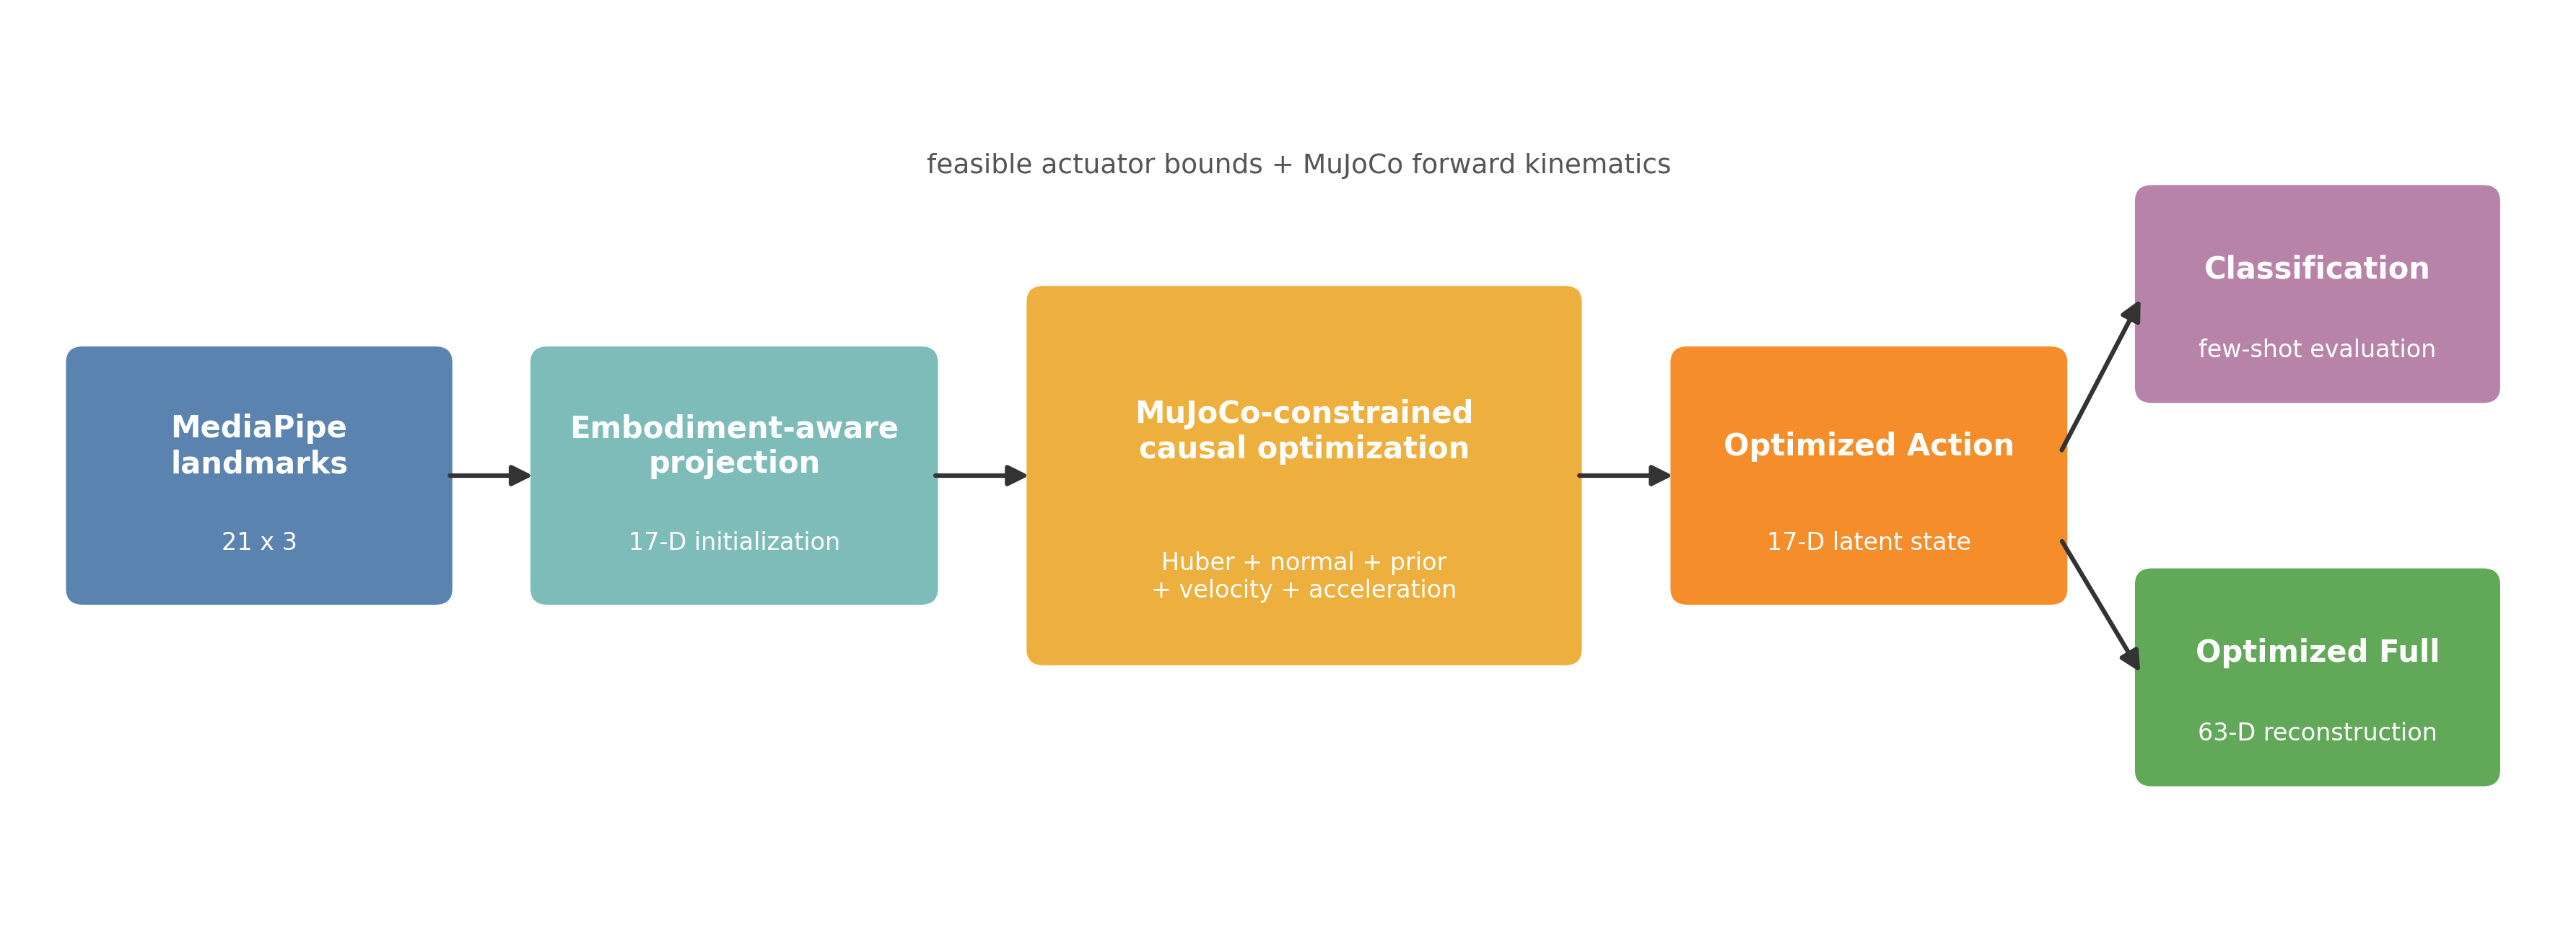
\includegraphics[width=\linewidth]{paper_updated_6class_20260820/method_pipeline.png}
\caption{Overview of the proposed refinement and evaluation pipeline. MediaPipe landmarks are first mapped to a 17-dimensional embodiment-aware initialization. Causal optimization then combines MuJoCo forward kinematics, actuator bounds, robust observation fitting, and temporal regularization. The resulting Optimized Action is used directly for recognition or reprojected as Optimized Full for landmark-space analysis.}
\label{fig:method_pipeline}
\end{figure}

\section{Pilot Experiments and Results}
The current experiments constitute a controlled pilot evaluation of representation quality. We first evaluate whether the proposed optimization improves frame-level stability and then test whether the refined latent representation benefits downstream sequence classification under limited supervision. These experiments are not intended to establish cross-subject or cross-session generalization.

\subsection{Controlled Dataset and Gesture Classes}
We evaluate the method on \url{gesture_sequence_dataset_chinese_dance_6class.csv}, a controlled six-class Chinese dance gesture subset filtered from the broader prototype collection. The six classes are \texttt{orchid\_palm}, \texttt{orchid\_finger}, \texttt{flower\_pinch}, \texttt{prayer\_beads}, \texttt{three\_finger\_bent}, and \texttt{deer\_horn}. This subset reflects the intended fine-grained application domain, but it is used here as an internal representation-analysis dataset rather than as a public benchmark.

Each sample is treated as one continuous labeled gesture clip rather than as a collection of independent frames. All frames belonging to a sequence remain together during splitting, preventing direct frame-level leakage between training and test sets. However, the current CSV does not contain participant or recording-session identifiers. The reported protocol is therefore sequence-disjoint but cannot be verified as subject-independent or session-independent. In contrast to larger gesture and skeleton benchmarks that define explicit cross-subject or cross-view protocols \cite{shahroudy2016ntu,caputo2021shrec,kopuklu2020drivermhg,kapitanov2022hagrid}, the present subset should be interpreted as a controlled prototype benchmark for representation analysis rather than evidence of population-level generalization.

The subset contains 571 gesture sequences and 26,260 frames. For each repeat, we first create a stratified sequence-level split with 20\% of the sequences held out for testing. We then retain three sequences per class from the remaining training partition, resulting in 18 training sequences and 115 test sequences in each repeat; unused candidates in the training partition do not enter model fitting. This process is repeated 20 times using seeds 42--61, and the same sequence split is used for every representation and classifier within a repeat. In this paper, \emph{few-shot} therefore refers operationally to a three-training-sequence-per-class supervised evaluation protocol; it does not denote episodic meta-learning. The classes are comparatively balanced at sequence level, but we retain macro-F1 and Cohen's kappa to expose class-dependent performance. The class distribution is summarized in Table~\ref{tab:dataset_summary}.

\begin{table}[!t]
\centering
\caption{Controlled six-class Chinese dance gesture subset used in the pilot experiments.}
\label{tab:dataset_summary}
\footnotesize
\begin{tabular}{@{}lcc@{}}
\toprule
Gesture label & Sequences & Frames \\
\midrule
\texttt{orchid\_palm} & 108 & 4613 \\
\texttt{orchid\_finger} & 92 & 4355 \\
\texttt{flower\_pinch} & 94 & 5013 \\
\texttt{prayer\_beads} & 92 & 4290 \\
\texttt{three\_finger\_bent} & 90 & 3869 \\
\texttt{deer\_horn} & 95 & 4120 \\
\midrule
Total & 571 & 26260 \\
\bottomrule
\end{tabular}
\end{table}

\begin{figure}[!t]
\centering

\includegraphics[width=0.86\linewidth]{paper_updated_6class_20260820/dataset_distribution_6class.png}
\caption{Class distribution of the updated controlled six-class Chinese dance gesture subset. Sequence counts are comparatively balanced, while frame counts reflect natural differences in gesture duration.}
\label{fig:dataset_distribution}
\end{figure}

\subsection{Frame-level Stability Evaluation}
Frame-level evaluation focuses on jitter, drift, and transient outliers. Beyond comparing raw landmarks, heuristic actuator projections, and optimized actuator states, we consider conventional temporal smoothing baselines, including moving average, Savitzky--Golay smoothing \cite{savitzky1964smoothing}, One-Euro filtering \cite{casiez2012oneeuro}, and Kalman filtering \cite{kalman1960new}, as simpler coordinate-space alternatives. These baselines test whether the observed benefits can be explained by landmark-space denoising alone.

We evaluate temporal smoothness separately in actuator space and landmark space. This distinction is important because the latent actuator trajectory and the reconstructed landmark trajectory live in different spaces, with different dimensionalities and scales. Within each space, lower velocity- and acceleration-based statistics indicate smoother temporal behavior.

\begin{table}[!t]
\centering
\caption{Actuator-space temporal stability on the six-class subset. Lower is better.}
\label{tab:jitter_actuator}
\small
\begin{tabular}{@{}lcccc@{}}
\toprule
Representation & Velocity Mean & Velocity RMS & Acceleration Mean & Acceleration RMS \\
\midrule
Corrected & 0.4590 & 0.6160 & 0.7100 & 0.9130 \\
Optimized Action & \textbf{0.2470} & \textbf{0.3109} & \textbf{0.2703} & \textbf{0.3396} \\
\bottomrule
\end{tabular}
\end{table}

\begin{table}[!t]
\centering
\caption{Landmark-space temporal stability on the six-class subset. Lower is better.}
\label{tab:jitter_landmark}
\footnotesize
\begin{tabular}{@{}lcccc@{}}
\toprule
Representation & Velocity Mean & Velocity RMS & Acceleration Mean & Acceleration RMS \\
\midrule
Raw & 0.6043 & 0.8002 & 0.7906 & 1.0070 \\
Moving Average & 0.3340 & 0.3983 & 0.1907 & 0.2332 \\
Savitzky--Golay & 0.4391 & 0.5292 & 0.2951 & 0.3514 \\
One-Euro & 0.3665 & 0.4526 & 0.2857 & 0.3711 \\
Kalman & \textbf{0.1737} & \textbf{0.2249} & \textbf{0.0974} & \textbf{0.1582} \\
Optimized Full & 0.3011 & 0.4143 & 0.3127 & 0.4168 \\
\bottomrule
\end{tabular}
\end{table}

\begin{figure}[!t]
\centering

\includegraphics[width=0.48\linewidth]{paper_updated_6class_20260820/jitter_actuator_6class.png}\hfill

\includegraphics[width=0.48\linewidth]{paper_updated_6class_20260820/jitter_landmark_6class.png}
\caption{Temporal stability summaries in actuator space and landmark space. The optimized actuator trajectory substantially reduces actuator-space velocity and acceleration relative to the heuristic corrected representation, while landmark-space reconstruction should be interpreted separately because it lives in a different coordinate space.}
\label{fig:jitter}
\end{figure}

Within actuator space, Optimized Action achieves lower velocity and acceleration than the heuristic Corrected representation, indicating that robust fitting and acceleration regularization suppress transient drift more effectively in the latent state trajectory. Within landmark space, conventional filters such as Kalman filtering can reduce coordinate variation more aggressively than the reconstructed MuJoCo landmarks. This does not contradict the recognition results below; rather, it shows that coordinate smoothness and discriminative representation quality are related but distinct evaluation criteria.

\begin{figure}[!t]
\centering
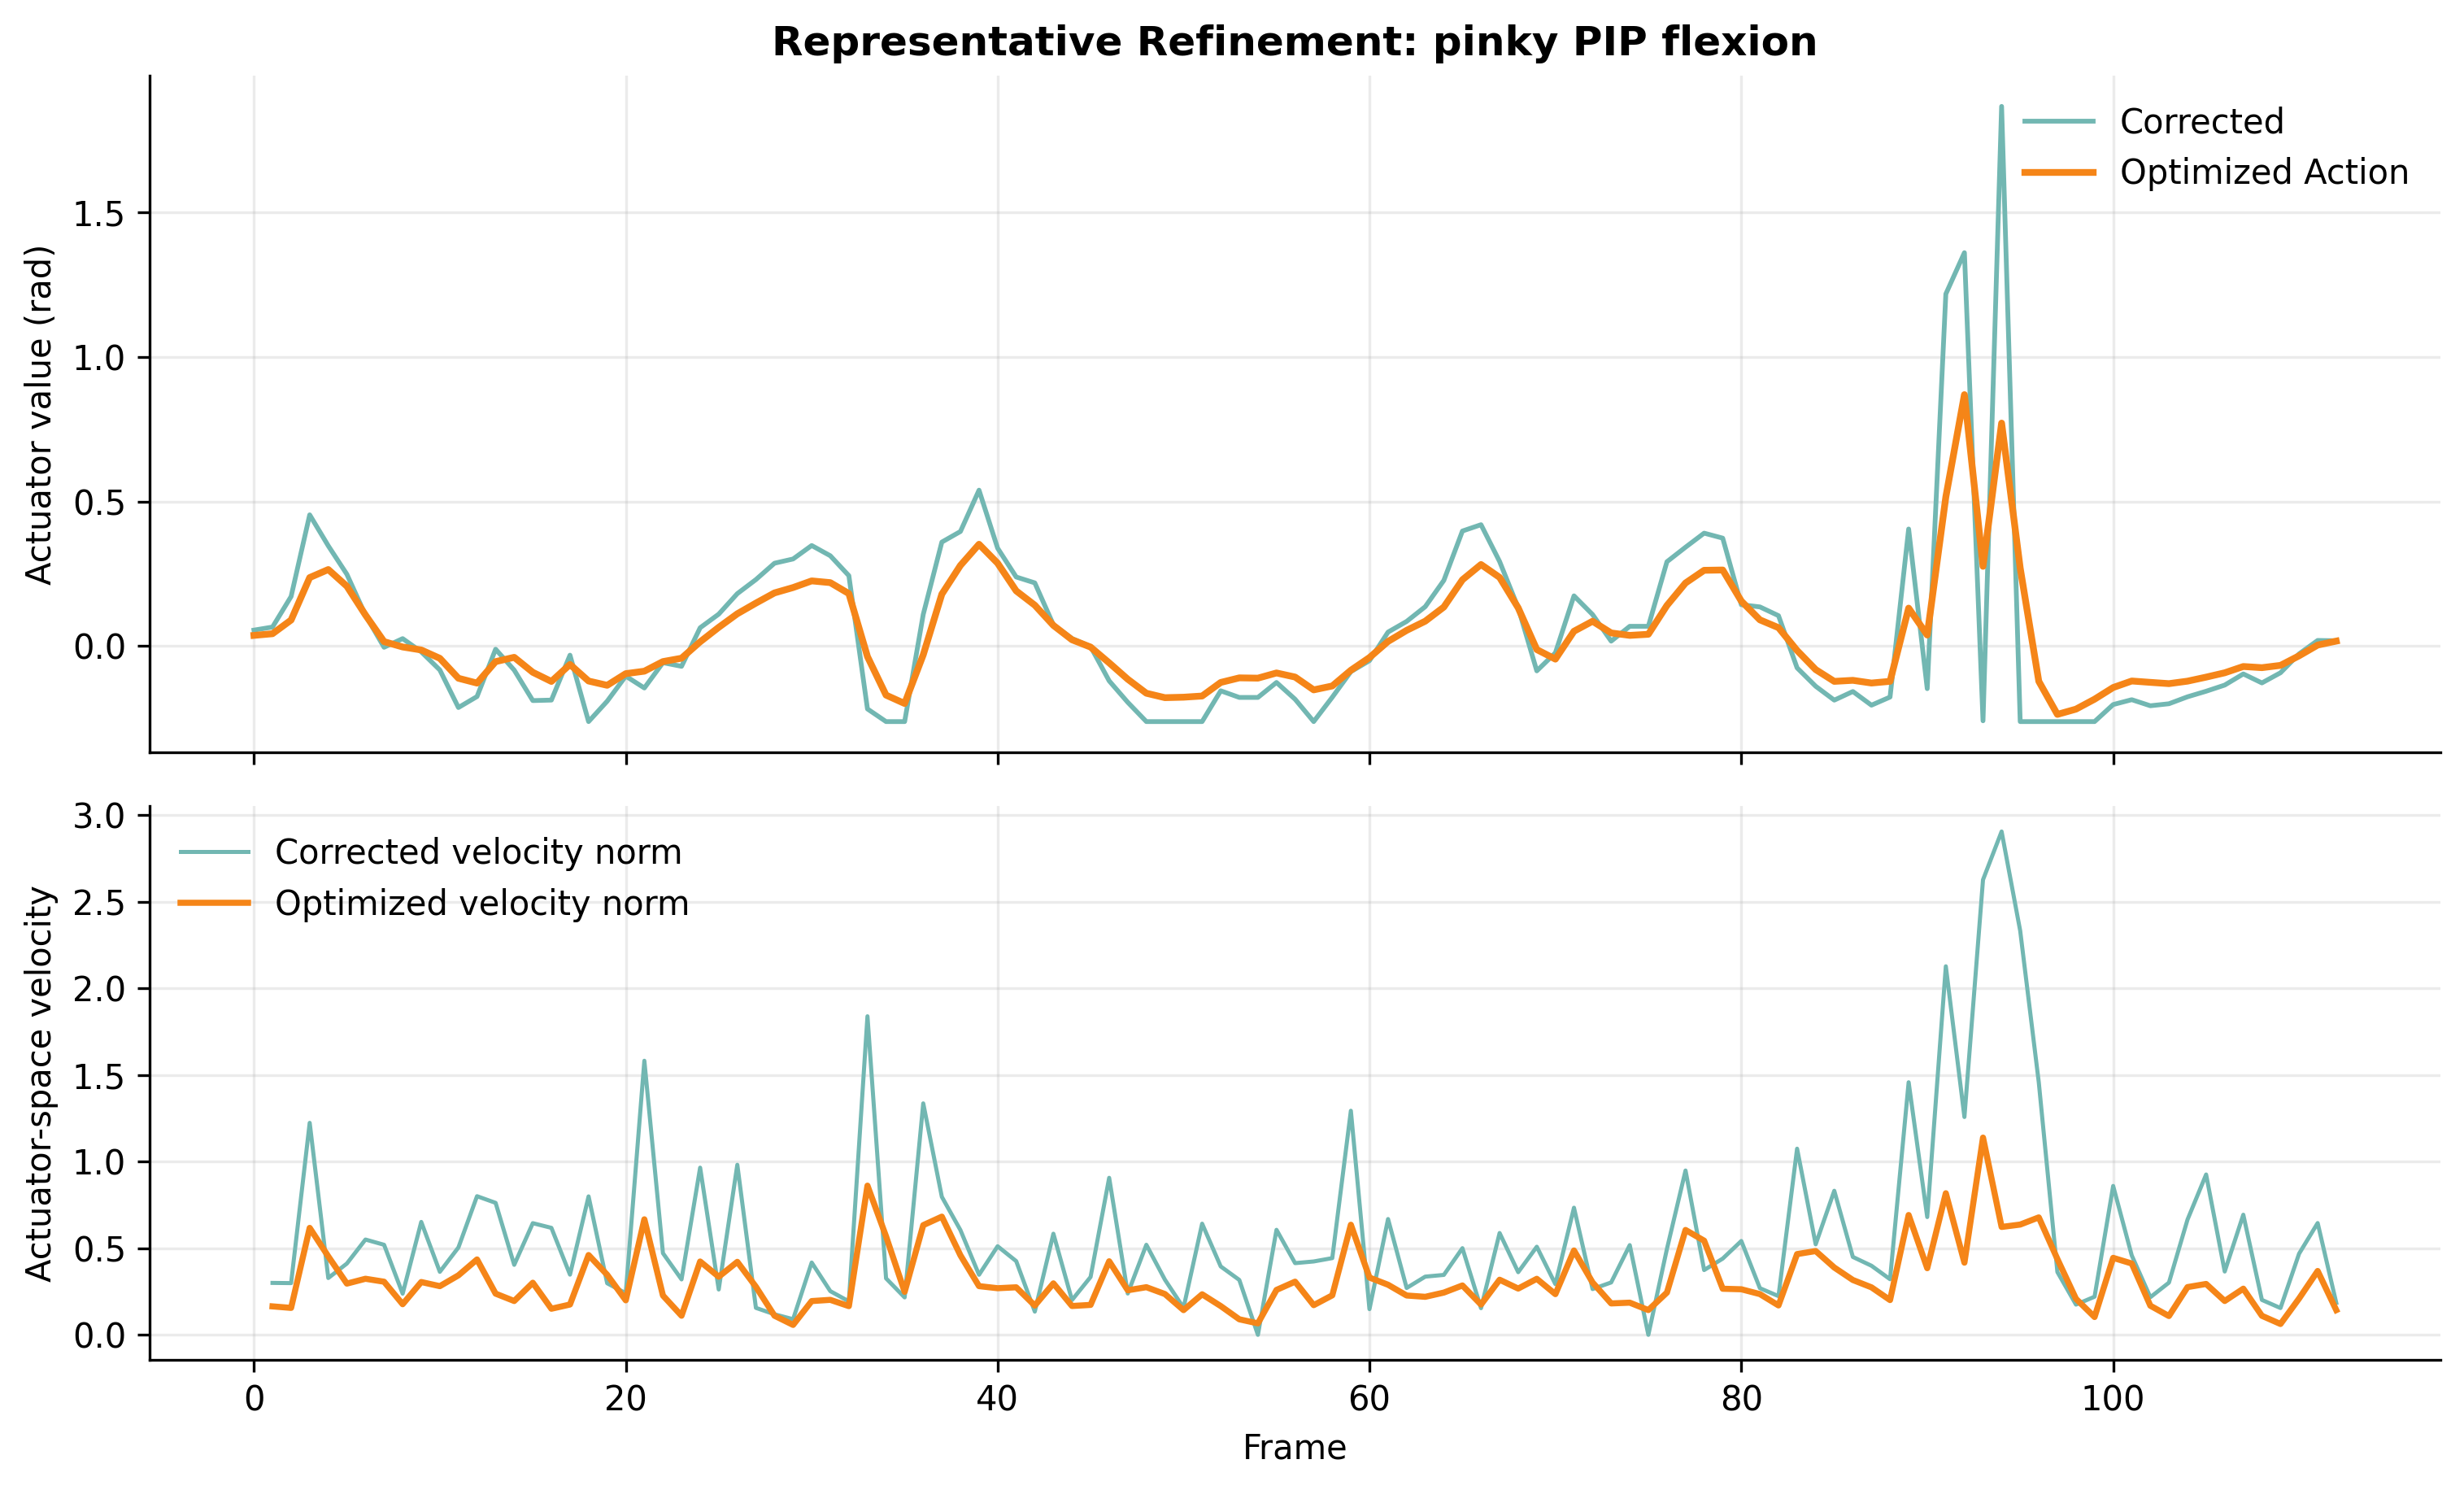
\includegraphics[width=0.94\linewidth]{paper_updated_6class_20260820/trajectory_refinement_example_6class.png}
\caption{Illustrative high-jitter sequence selected by the largest reduction in maximum second-order actuator change. The upper panel shows the pinky PIP trajectory before and after MuJoCo-constrained refinement; the lower panel shows the full actuator-space velocity norm. The example visualizes how isolated peaks are attenuated without forcing the trajectory to remain constant.}
\label{fig:trajectory_example}
\end{figure}

\subsection{Sequence-level Three-shot Classification}
To measure downstream utility, we aggregate frame-level features into sequence descriptors and train ordinary lightweight classifiers under the three-shot protocol defined above. The classifiers themselves are not few-shot or meta-learning algorithms; the low-shot condition is imposed by limiting their supervised training data to three sequences per class. Standardization is fitted only on each repeat's training descriptors and then applied to the corresponding test descriptors. For PCA experiments, both frame-level standardization and PCA are fitted exclusively on training frames before transforming and aggregating the test sequences. The key question is whether a temporally stable actuator trajectory is more discriminative than raw landmark coordinates under limited training data. The representation comparisons are organized in two stages. First, we compare against simple filtering baselines to examine whether ordinary temporal smoothing is sufficient. Second, we compare against PCA-reduced baselines to examine whether the gains from actuator-space representations can be explained by generic dimensionality reduction.

Table~\ref{tab:main_classifiers} reports the updated six-class results across four lightweight classifiers. Both actuator-space representations substantially outperform Raw and Optimized Full under every classifier. Corrected gives the highest mean recognition performance, with RandomForest reaching $0.7826 \pm 0.0611$ accuracy, $0.7803 \pm 0.0677$ macro-F1, and $0.7393 \pm 0.0733$ Cohen's kappa. Optimized Action remains close at $0.7674 \pm 0.0626$ accuracy while providing much lower actuator-space temporal variation. The enlarged evaluation therefore reveals a stability--discrimination trade-off that was not visible in the smaller pilot subset.

\begin{table}[!t]
\centering
\caption{Sequence classification results on the controlled six-class Chinese dance subset. Results are mean $\pm$ standard deviation over 20 repeated three-shot supervised splits.}
\label{tab:main_classifiers}
\scriptsize
\begin{tabular}{@{}llccc@{}}
\toprule
Classifier & Representation & Accuracy & Macro-F1 & Kappa \\
\midrule
\multirow{4}{*}{SVM}
& Raw & $0.3887 \pm 0.0380$ & $0.3761 \pm 0.0396$ & $0.2664 \pm 0.0461$ \\
& Corrected & $\mathbf{0.7491 \pm 0.0639}$ & $\mathbf{0.7543 \pm 0.0632}$ & $\mathbf{0.6988 \pm 0.0769}$ \\
& Optimized Action & $0.7278 \pm 0.0536$ & $0.7320 \pm 0.0519$ & $0.6732 \pm 0.0645$ \\
& Optimized Full & $0.4578 \pm 0.0766$ & $0.4546 \pm 0.0767$ & $0.3497 \pm 0.0911$ \\
\midrule
\multirow{4}{*}{KNN}
& Raw & $0.3543 \pm 0.0517$ & $0.3360 \pm 0.0586$ & $0.2244 \pm 0.0619$ \\
& Corrected & $\mathbf{0.7030 \pm 0.0733}$ & $\mathbf{0.6986 \pm 0.0765}$ & $\mathbf{0.6438 \pm 0.0879}$ \\
& Optimized Action & $0.6804 \pm 0.0641$ & $0.6741 \pm 0.0665$ & $0.6168 \pm 0.0766$ \\
& Optimized Full & $0.4152 \pm 0.0638$ & $0.4058 \pm 0.0683$ & $0.2989 \pm 0.0756$ \\
\midrule
\multirow{4}{*}{RandomForest}
& Raw & $0.4309 \pm 0.0442$ & $0.4145 \pm 0.0420$ & $0.3163 \pm 0.0536$ \\
& Corrected & $\mathbf{0.7826 \pm 0.0611}$ & $\mathbf{0.7803 \pm 0.0677}$ & $\mathbf{0.7393 \pm 0.0733}$ \\
& Optimized Action & $0.7674 \pm 0.0626$ & $0.7632 \pm 0.0666$ & $0.7211 \pm 0.0750$ \\
& Optimized Full & $0.5061 \pm 0.0921$ & $0.4973 \pm 0.0903$ & $0.4078 \pm 0.1102$ \\
\midrule
\multirow{4}{*}{MLP}
& Raw & $0.3922 \pm 0.0504$ & $0.3785 \pm 0.0488$ & $0.2703 \pm 0.0607$ \\
& Corrected & $\mathbf{0.7478 \pm 0.0716}$ & $\mathbf{0.7477 \pm 0.0750}$ & $\mathbf{0.6975 \pm 0.0858}$ \\
& Optimized Action & $0.7330 \pm 0.0692$ & $0.7326 \pm 0.0705$ & $0.6798 \pm 0.0828$ \\
& Optimized Full & $0.4574 \pm 0.0765$ & $0.4518 \pm 0.0811$ & $0.3490 \pm 0.0917$ \\
\bottomrule
\end{tabular}
\end{table}

Because all representations use identical train/test sequence IDs in each repeat, their results can also be compared as paired observations. Figure~\ref{fig:paired_accuracy} shows the repeat-wise accuracy difference between Optimized Action and the two actuator-pipeline baselines. Relative to Raw, the mean gains are 0.3391, 0.3261, 0.3365, and 0.3409 for SVM, KNN, RandomForest, and MLP, respectively; Optimized Action is higher in all 20 repeats for every classifier. Relative to Corrected, however, the mean differences are $-0.0213$, $-0.0226$, $-0.0152$, and $-0.0148$. The differences favor Corrected significantly for SVM, KNN, and RandomForest in the exploratory Wilcoxon tests, but not for MLP. Thus, the optimization retains a large benefit over unstructured observations but does not improve recognition over its heuristic initialization on the enlarged dataset. Because repeated holdout splits overlap and are not statistically independent, these $p$-values remain exploratory rather than definitive population-level significance tests.

\begin{table}[!t]
\centering
\caption{Exploratory paired accuracy comparison for Optimized Action using identical repeated splits. Positive/equal/negative counts indicate the number of repeats in which Optimized Action performs better than, equal to, or worse than the baseline. The Wilcoxon values should be interpreted with caution because repeated holdout splits overlap.}
\label{tab:paired_accuracy}
\footnotesize
\begin{tabular}{@{}llcccc@{}}
\toprule
Classifier & Baseline & Mean $\Delta$ accuracy & Positive / Equal / Negative & Wilcoxon $p$ \\
\midrule
SVM & Raw & +0.3391 & 20 / 0 / 0 & $<0.001$ \\
SVM & Corrected & $-0.0213$ & 5 / 0 / 15 & 0.0045 \\
KNN & Raw & +0.3261 & 20 / 0 / 0 & $<0.001$ \\
KNN & Corrected & $-0.0226$ & 3 / 2 / 15 & 0.0040 \\
RandomForest & Raw & +0.3365 & 20 / 0 / 0 & $<0.001$ \\
RandomForest & Corrected & $-0.0152$ & 5 / 2 / 13 & 0.0058 \\
MLP & Raw & +0.3409 & 20 / 0 / 0 & $<0.001$ \\
MLP & Corrected & $-0.0148$ & 5 / 2 / 13 & 0.1061 \\
\bottomrule
\end{tabular}
\end{table}

\begin{figure}[!t]
\centering

\includegraphics[width=0.96\linewidth]{paper_updated_6class_20260820/paired_accuracy_improvement_6class.png}
\caption{Paired accuracy differences across the same 20 three-shot supervised sequence splits. Values above zero favor Optimized Action. The refined representation consistently exceeds Raw but is slightly below the frame-independent Corrected representation, exposing the stability--discrimination trade-off.}
\label{fig:paired_accuracy}
\end{figure}

\subsection{Comparison with Conventional Smoothing Baselines}
To determine whether the classification gains can be explained by ordinary coordinate-space denoising, we compare raw landmarks, four conventional temporal filters, and the proposed structured representations using the same RandomForest three-shot protocol. Each result is reported as mean $\pm$ standard deviation over 20 repeated three-shot splits. The smoothing baselines are moving average, Savitzky--Golay, One-Euro, and Kalman filtering.

\begin{table}[H]
\centering
\caption{RandomForest three-shot classification comparison between conventional landmark-space smoothing and structured ORCA/MuJoCo representations. Results are mean $\pm$ standard deviation over 20 repeated sequence-level splits.}
\label{tab:smoothing_baselines}
\footnotesize
\begin{tabular}{@{}lccc@{}}
\toprule
Representation & Accuracy & Macro-F1 & Kappa \\
\midrule
Raw & $0.4309 \pm 0.0442$ & $0.4145 \pm 0.0420$ & $0.3163 \pm 0.0536$ \\
Moving Average & $0.4248 \pm 0.0485$ & $0.4088 \pm 0.0497$ & $0.3089 \pm 0.0596$ \\
Savitzky--Golay & $0.4204 \pm 0.0432$ & $0.4053 \pm 0.0464$ & $0.3036 \pm 0.0528$ \\
One-Euro & $0.4187 \pm 0.0544$ & $0.4022 \pm 0.0530$ & $0.3020 \pm 0.0666$ \\
Kalman & $0.4096 \pm 0.0447$ & $0.3966 \pm 0.0432$ & $0.2914 \pm 0.0545$ \\
Corrected & $\mathbf{0.7826 \pm 0.0611}$ & $\mathbf{0.7803 \pm 0.0677}$ & $\mathbf{0.7393 \pm 0.0733}$ \\
Optimized Action & $0.7674 \pm 0.0626$ & $0.7632 \pm 0.0666$ & $0.7211 \pm 0.0750$ \\
Optimized Full & $0.5061 \pm 0.0921$ & $0.4973 \pm 0.0903$ & $0.4078 \pm 0.1102$ \\
\bottomrule
\end{tabular}
\end{table}

\begin{figure}[!htbp]
\centering

\includegraphics[width=0.88\linewidth]{paper_updated_6class_20260820/smoothing_baselines_6class.png}
\caption{RandomForest accuracy comparison between conventional landmark-space smoothing baselines and structured actuator representations. Conventional smoothing reduces jitter but does not improve recognition, while Corrected and Optimized Action retain substantially more discriminative information.}
\label{fig:smoothing_baselines}
\end{figure}

The results show that conventional smoothing does not translate into stronger recognition on the updated dataset. Every coordinate filter reduces RandomForest accuracy relative to Raw, and Kalman filtering, despite producing the lowest landmark-space velocity and acceleration, gives the lowest mean accuracy among the coordinate baselines. Corrected and Optimized Action instead improve accuracy by 0.3517 and 0.3365 over Raw, respectively. Read together with the jitter analysis, this is an important result: aggressively reducing coordinate variation is neither necessary nor sufficient for preserving gesture-discriminative articulation. The benefit of actuator-space representation therefore cannot be attributed to ordinary coordinate smoothing alone.

\FloatBarrier
\subsection{Classifier Comparison}
The classifier comparison suggests two complementary observations. First, representation choice matters strongly: all four classifiers improve substantially when moving from raw landmarks to structured actuator-space features. Second, the broad ranking is classifier-independent: Corrected ranks first and Optimized Action second for SVM, KNN, RandomForest, and MLP. RandomForest gives the strongest mean result for both actuator representations. The optimization is therefore best understood as trading a small amount of class separation for a large reduction in temporal variation, rather than as an unconditional classification improvement over its initialization.

\begin{figure}[!htbp]
\centering

\includegraphics[width=\linewidth]{paper_updated_6class_20260820/performance_heatmaps_6class.png}
\caption{Mean accuracy, macro-F1, and Cohen's kappa across classifiers and non-PCA representations. Corrected has the highest recognition score in every classifier column, while Optimized Action remains close and is temporally smoother. Optimized Full loses discriminative information after reconstruction into the higher-dimensional landmark space.}
\label{fig:classifier_suite}
\end{figure}

Figure~\ref{fig:confusion} separates the contributions of heuristic projection and MuJoCo optimization under SVM. Most of the gain over Raw is obtained by entering the structured actuator space. The additional optimization changes the remaining errors in a class-dependent manner but does not improve aggregate recognition over Corrected. This pattern reinforces the distinction between temporal stabilization and class separation.

\begin{figure}[!t]
\centering

\includegraphics[width=\linewidth]{paper_updated_6class_20260820/cm_svm_representation_stages_6class.png}
\caption{Aggregate SVM confusion matrices across all 20 repeats for Raw, Corrected, and Optimized Action. Actuator-space projection provides the dominant recognition gain; MuJoCo-constrained refinement substantially stabilizes the trajectory but introduces small class-dependent recognition losses.}
\label{fig:confusion}
\end{figure}

\FloatBarrier
\subsection{Loss Ablation}
\label{sec:loss_ablation}
We evaluate five targeted variants without retuning the remaining weights: removal of palm-normal alignment, removal of acceleration regularization, removal of both temporal terms, and replacement of component-wise Huber fitting with squared $L_2$ residuals. Corrected is included as the no-optimization reference. All variants use the same observations and the same saved sequence splits as the full method.

\begin{table}[!t]
\centering
\caption{Loss ablation in actuator space. Stability values are averaged over 571 sequences; classification values are mean $\pm$ standard deviation over the same 20 three-shot supervised splits. Lower stability values indicate smoother trajectories.}
\label{tab:loss_ablation}
\scriptsize
\begin{tabular}{@{}lcccc@{}}
\toprule
Variant & Velocity mean & Acceleration mean & SVM accuracy & RF accuracy \\
\midrule
Corrected only & 0.4590 & 0.7100 & $\mathbf{0.7491\pm0.0639}$ & $\mathbf{0.7826\pm0.0611}$ \\
Full & 0.2470 & 0.2703 & $0.7278\pm0.0536$ & $0.7674\pm0.0626$ \\
Without palm normal & \textbf{0.2391} & \textbf{0.2646} & $0.7378\pm0.0587$ & $0.7717\pm0.0508$ \\
Without acceleration & 0.2685 & 0.3718 & $0.7213\pm0.0568$ & $0.7730\pm0.0606$ \\
Without temporal terms & 0.3238 & 0.4976 & $0.7096\pm0.0543$ & $0.7609\pm0.0693$ \\
$L_2$ instead of Huber & 0.2560 & 0.2926 & $0.6548\pm0.0824$ & $0.7335\pm0.0633$ \\
\bottomrule
\end{tabular}
\end{table}

\begin{figure}[!t]
\centering

\includegraphics[width=\linewidth]{paper_updated_6class_20260820/loss_ablation_stability_tradeoff_6class.png}
\caption{Loss ablation separates temporal stability from recognition performance. Temporal regularization markedly reduces actuator velocity and acceleration, but the smoothest or most strongly regularized trajectory is not necessarily the most discriminative under the current classifier protocol.}
\label{fig:loss_ablation}
\end{figure}

Removing acceleration increases mean second-order variation from 0.2703 to 0.3718, while removing both temporal terms increases it to 0.4976. Thus, the temporal losses perform their intended stabilization role. The full method also exceeds the no-temporal variant by 0.0183 SVM accuracy ($p=0.0006$), although its RandomForest difference is small and non-significant. Removing palm-normal alignment produces slightly smoother trajectories and changes recognition only modestly: it is 0.0100 higher than Full under SVM ($p=0.0494$) and 0.0043 higher under RandomForest ($p=0.4686$). Palm alignment is therefore best justified as a model-consistency term rather than by an observed classification gain. The clearest discriminative component is robust fitting. Replacing Huber with $L_2$ lowers SVM and RandomForest accuracy by 0.0730 and 0.0339, respectively, and increases mean solve time from 27.6 to 74.9 ms per frame. The ablation supports Huber fitting and temporal stabilization while showing that the current palm weight and overall stability--discrimination balance warrant future validation.

\FloatBarrier
\subsection{Dimension-matched PCA Baseline}
Because Optimized Action is 17-dimensional, we compare it with PCA-17 fitted exclusively on the training frames of each repeat \cite{jolliffe2002pca}. The transformed frames are aggregated only after PCA fitting, and every representation uses identical train/test sequence IDs. Table~\ref{tab:pca_comparison} reports matched classifier comparisons rather than mixing the best result from different classifiers.

\begin{table}[!t]
\centering
\caption{Accuracy for the dimension-matched PCA comparison. Values are means over 20 repeated three-shot sequence splits. Bold marks the best representation within each classifier.}
\label{tab:pca_comparison}
\footnotesize
\begin{tabular}{@{}lcccc@{}}
\toprule
Representation & SVM & KNN & RandomForest & MLP \\
\midrule
Raw & 0.3887 & 0.3543 & 0.4309 & 0.3922 \\
PCA-17 & 0.6339 & 0.5822 & 0.6543 & 0.6191 \\
Corrected & \textbf{0.7491} & \textbf{0.7030} & \textbf{0.7826} & \textbf{0.7478} \\
Optimized Action & 0.7278 & 0.6804 & 0.7674 & 0.7330 \\
Optimized Full & 0.4578 & 0.4152 & 0.5061 & 0.4574 \\
\bottomrule
\end{tabular}
\end{table}

\begin{figure}[!t]
\centering

\includegraphics[width=\linewidth]{paper_updated_6class_20260820/pca_all_classifiers_6class.png}
\caption{Accuracy and macro-F1 for PCA-17 and structured representations under all four classifiers. Both actuator representations consistently exceed dimension-matched PCA-17, showing that their benefit is not explained by dimensionality reduction alone.}
\label{fig:pca_comparison}
\end{figure}

The PCA comparison provides stronger evidence than the smaller pilot experiment. Corrected and Optimized Action exceed PCA-17 under all four classifiers, with Optimized Action improving over PCA-17 by 0.0939--0.1261 accuracy points depending on the classifier. Dimensionality reduction alone therefore does not explain the actuator-space advantage. At the same time, Corrected remains slightly more discriminative than Optimized Action, indicating that the temporal objective does not preserve every class-relevant variation in the heuristic projection.

\subsection{Training-size Sensitivity}
The primary evaluation fixes the training budget at three sequences per class. We additionally sweep 1, 3, 5, and 10 training sequences per class to determine whether the representation ranking is specific to this choice while remaining within the intended low-data regime. Within each of 20 repeats, a stratified 20\% test partition is held fixed and the training subsets are nested, so the smaller training set is always contained in the larger one. This sweep uses a separately generated nested manifest; consequently, its three-shot estimates are close to, but not identical to, the primary results in Table~\ref{tab:main_classifiers}.

\begin{table}[!t]
\centering
\caption{RandomForest accuracy as the number of training sequences per class increases. Each entry is the mean over 20 repeated nested splits.}
\label{tab:shot_sweep}
\footnotesize
\begin{tabular}{@{}rrrrrr@{}}
\toprule
Shot & Total train & Raw & PCA-17 & Corrected & Optimized Action \\
\midrule
1  & 6   & 0.2878 & 0.3939 & \textbf{0.5417} & 0.5296 \\
3  & 18  & 0.4187 & 0.6687 & \textbf{0.7748} & 0.7683 \\
5  & 30  & 0.5239 & 0.7743 & \textbf{0.8561} & 0.8491 \\
10 & 60  & 0.6813 & 0.8874 & \textbf{0.9048} & 0.9013 \\
\bottomrule
\end{tabular}
\end{table}

\begin{figure}[!t]
\centering

\includegraphics[width=\linewidth]{paper_updated_6class_20260820/shot_sweep_accuracy_6class.png}
\caption{Accuracy learning curves for all four classifiers over the 1--10-shot range. Error bars show 95\% confidence intervals over 20 repeated nested splits. The actuator representations consistently outperform Raw and PCA-17 throughout the intended low-data regime.}
\label{fig:shot_sweep_accuracy}
\end{figure}

\begin{figure}[!t]
\centering

\includegraphics[width=\linewidth]{paper_updated_6class_20260820/shot_sweep_macro_f1_6class.png}
\caption{Macro-F1 learning curves under the same shot sweep. The similar accuracy and macro-F1 trends indicate that the low-shot gains are not caused only by the class distribution.}
\label{fig:shot_sweep_f1}
\end{figure}

The sweep demonstrates that the three-shot finding is not an isolated consequence of one training budget. Under RandomForest, the 1-shot accuracies of Corrected and Optimized Action are 0.5417 and 0.5296, compared with 0.2878 for Raw and 0.3939 for PCA-17. At 10-shot, Corrected and Optimized Action reach 0.9048 and 0.9013, while Raw and PCA-17 reach 0.6813 and 0.8874. Both actuator representations therefore retain an advantage throughout the tested low-data range. Corrected remains slightly more discriminative, whereas Optimized Action supplies the substantially smoother trajectory established by the stability evaluation. The complete RandomForest confusion matrices for all four training budgets and four principal representations are provided in Figure~\ref{fig:shot_cm_representations_appendix}.

\FloatBarrier
\section{Discussion}
\subsection{Why Structured Refinement Improves Sequence Classification}
Sequence classifiers depend on stable frame-level evidence. When raw landmarks fluctuate because of viewpoint changes or self-occlusion, the resulting sequence descriptors mix gesture information with estimation noise. The smoothing comparison in Table~\ref{tab:smoothing_baselines} clarifies that coordinate-space smoothness and discriminative representation quality are related but not equivalent.

All four conventional filters reduce RandomForest recognition relative to Raw even though they substantially reduce landmark-space velocity and acceleration. Kalman filtering is the clearest example: it produces the lowest landmark-space jitter but reaches only $0.4096 \pm 0.0447$ accuracy. In contrast, Corrected and Optimized Action reach $0.7826 \pm 0.0611$ and $0.7674 \pm 0.0626$, respectively. This suggests that the benefit of the ORCA representations is not simply a result of suppressing coordinate-space jitter. Instead, the actuator parameterization removes nuisance variation while retaining articulation cues that are useful for distinguishing the six gestures.

\subsection{Reconstruction versus Discriminative Representation}
A lower reconstruction error does not necessarily imply better classification. The reconstructed landmark space Optimized Full is useful for visualization and kinematic plausibility checks, but both compact actuator representations are more attractive for few-shot classification because they are lower-dimensional, structured, and semantically aligned with hand articulation.

The PCA comparison provides a second clarification. Even if a compact representation improves classification, that improvement is not automatically evidence for embodiment-aware representation, because generic dimensionality reduction can also help in low-data settings. Both Corrected and Optimized Action exceed PCA-17 for every classifier at the primary three-shot budget and remain ahead throughout the 1--10-shot sensitivity range. The evidence therefore supports actuator space as a useful low-data inductive bias. It does not show that the temporal optimizer is always preferable to its initialization: Corrected is the strongest classifier input in most conditions, whereas Optimized Action is the more stable trajectory.

\subsection{Stability versus Discrimination}
The loss ablation demonstrates that temporal smoothness and downstream discrimination are not interchangeable objectives. Acceleration and first-order temporal penalties substantially reduce actuator-space variation, and removing both temporal terms also lowers SVM recognition, but Corrected still classifies slightly better than the smoother Full trajectory. Huber fitting is important for both classifiers and is much faster than the tested squared-residual alternative. Palm-normal alignment does not improve classification in this dataset and slightly increases variation relative to the no-palm variant; its present value is kinematic orientation consistency. Future parameter selection should therefore consider recovery, stability, and downstream recognition jointly rather than optimizing any one criterion in isolation.

\subsection{Answers to the Research Questions}
\textbf{RQ1: Temporal stability.} Within actuator space, Optimized Action reduces mean velocity from 0.4590 to 0.2470 and mean acceleration from 0.7100 to 0.2703 relative to Corrected. The current evidence therefore indicates that the refinement performs its intended stabilization role.

\textbf{RQ2: Downstream recognition.} Within the current repeated sequence splits, Optimized Action improves mean accuracy over Raw for SVM, KNN, RandomForest, and MLP. This is evidence of within-domain representation utility, not yet of cross-subject or cross-session generalization.

\textbf{RQ3: Simpler explanations.} The result cannot be explained by smoothing or dimensionality reduction alone within the tested low-data regime. Kalman filtering produces the lowest landmark-space velocity and acceleration but lowers recognition relative to Raw, while PCA-17 remains below both actuator representations under every classifier at three-shot and throughout the 1--10-shot sweep.

\textbf{RQ4: Component roles and cost.} Temporal regularization strongly improves stability and supports SVM recognition relative to removing both temporal terms. Huber fitting improves both tested classifiers and is substantially faster than the $L_2$ alternative. Palm-normal alignment enforces orientation consistency but does not produce a recognition gain in the updated ablation. The full solver requires 27.6 ms per frame on average and 32.6 ms at the 95th percentile in the reported CPU benchmark; these observations do not imply that the current fixed weights are globally optimal.

\subsection{Limitations}
The current evaluation uses lightweight statistical sequence aggregation, which is convenient and interpretable but discards temporal ordering beyond low-order summaries. More importantly, the CSV does not encode participant or session identity, so the sequence-disjoint results cannot establish cross-subject or cross-session generalization. Although the updated dataset is much larger and comparatively balanced, repeated holdout tests still reuse overlapping samples; their $p$-values are therefore exploratory rather than independent population-level significance tests. The trajectory in Figure~\ref{fig:trajectory_example} was deliberately selected as a high-jitter diagnostic example and should not be interpreted as an unbiased estimate of average visual improvement. The coordinate alignment translates and scales the hand but does not yet construct a fully canonical palm-local frame. Finally, the small recognition loss from Corrected to Optimized Action shows that the fixed temporal weights may suppress some gesture-relevant variation.

\subsection{Future Work}
The immediate next step is subject- and session-annotated data collection followed by group-disjoint evaluation. Stronger temporal encoders can then test whether the refined actuator trajectory remains useful when sequence order is modeled explicitly. A separate extension is confidence-aware refinement: per-landmark reliability estimates could reduce the observation weight of an occluded finger and increase reliance on a learned temporal prior. We deliberately leave that learned, adaptive formulation outside the scope of the present fixed-weight method. Fusion of PCA-compressed landmark cues with Optimized Action is another promising direction because the two representations preserve complementary information.

\section{Conclusion}
We presented a fixed-weight causal MuJoCo-constrained framework for refining MediaPipe observations in ORCA actuator space. On the updated 571-sequence six-class dataset, Optimized Action improves substantially over raw landmarks and PCA-17 in the primary three-shot evaluation across four lightweight classifiers while reducing actuator-space mean velocity by 46.2\% and mean acceleration by 61.9\% relative to Corrected. Corrected nevertheless gives the highest classification performance in most conditions, revealing that stronger temporal stability can come at a small cost in discrimination. A nested 1--10-shot sensitivity analysis confirms that both actuator representations retain their advantage over Raw and PCA-17 throughout the intended low-data regime. Conventional filters reinforce the distinction between smoothness and recognition: Kalman filtering gives the smoothest landmark trajectory but lowers three-shot recognition relative to Raw. Optimized Full further confirms that reconstructing a higher-dimensional landmark representation is not automatically beneficial. These findings support a structured, interpretable, and sample-efficient representation-level contribution and identify stability--discrimination balance as the main limitation of the fixed-weight optimizer. Subject- and session-disjoint experiments remain necessary before making general claims about Chinese dance gesture recognition.

\appendix
\section{Additional Diagnostic Figures}

Figure~\ref{fig:per_class_recall_appendix} reports per-class SVM recall in a format complementary to the confusion matrices. Figure~\ref{fig:all_classifier_cm_appendix} shows that the remaining errors under Optimized Action depend on the downstream classifier. Figures~\ref{fig:shot_cm_progression_appendix}--\ref{fig:shot_recall_appendix} show how class-level errors change with the training budget. Figure~\ref{fig:ablation_accuracy_appendix} provides the classification-only view of the loss ablation, and Figure~\ref{fig:implementation_validation_appendix} summarizes the palm-normal consistency regression test and synthetic recovery check used to validate the implementation.

\begin{figure}[!t]
\centering

\includegraphics[width=0.94\linewidth]{paper_updated_6class_20260820/per_class_recall_svm_6class.png}
\caption{Per-class SVM recall across Raw, Corrected, and Optimized Action. The largest gains over Raw occur for flower pinch, orchid finger, and three-finger bent, whereas deer horn remains difficult.}
\label{fig:per_class_recall_appendix}
\end{figure}

\begin{figure}[!t]
\centering

\includegraphics[width=0.88\linewidth]{paper_updated_6class_20260820/cm_optimized_action_all_classifiers_6class.png}
\caption{Aggregate confusion matrices for Optimized Action under all four classifiers.}
\label{fig:all_classifier_cm_appendix}
\end{figure}

\begin{figure}[!t]
\centering

\includegraphics[width=\linewidth]{paper_updated_6class_20260820/cm_shot_progression_rf_optimized_action_6class.png}
\caption{Aggregate RandomForest confusion matrices for Optimized Action from 1-shot to 10-shot. Class-specific confusion decreases substantially as the number of labeled sequences increases.}
\label{fig:shot_cm_progression_appendix}
\end{figure}

\begin{figure}[p]
\centering

\includegraphics[width=\textwidth,height=0.88\textheight,keepaspectratio]{paper_updated_6class_20260820/cm_low_vs_high_shot_rf_representations_6class.png}
\caption{RandomForest confusion matrices for Raw, PCA-17, Corrected, and Optimized Action at 1, 3, 5, and 10 shots per class. Rows show increasing training budgets and columns show representation choices. Both actuator representations retain an advantage across the tested low-data range.}
\label{fig:shot_cm_representations_appendix}
\end{figure}

\begin{figure}[!t]
\centering

\includegraphics[width=0.96\linewidth]{paper_updated_6class_20260820/shot_sweep_per_class_recall_rf_6class.png}
\caption{Per-class RandomForest recall across shot counts for Corrected and Optimized Action. Orchid palm remains the most difficult 10-shot class for Optimized Action.}
\label{fig:shot_recall_appendix}
\end{figure}

\begin{figure}[!t]
\centering

\includegraphics[width=0.94\linewidth]{paper_updated_6class_20260820/loss_ablation_6class.png}
\caption{SVM and RandomForest accuracy for the targeted loss ablations. Error bars show standard deviation over the same 20 repeated three-shot supervised sequence splits.}
\label{fig:ablation_accuracy_appendix}
\end{figure}

\begin{figure}[!t]
\centering
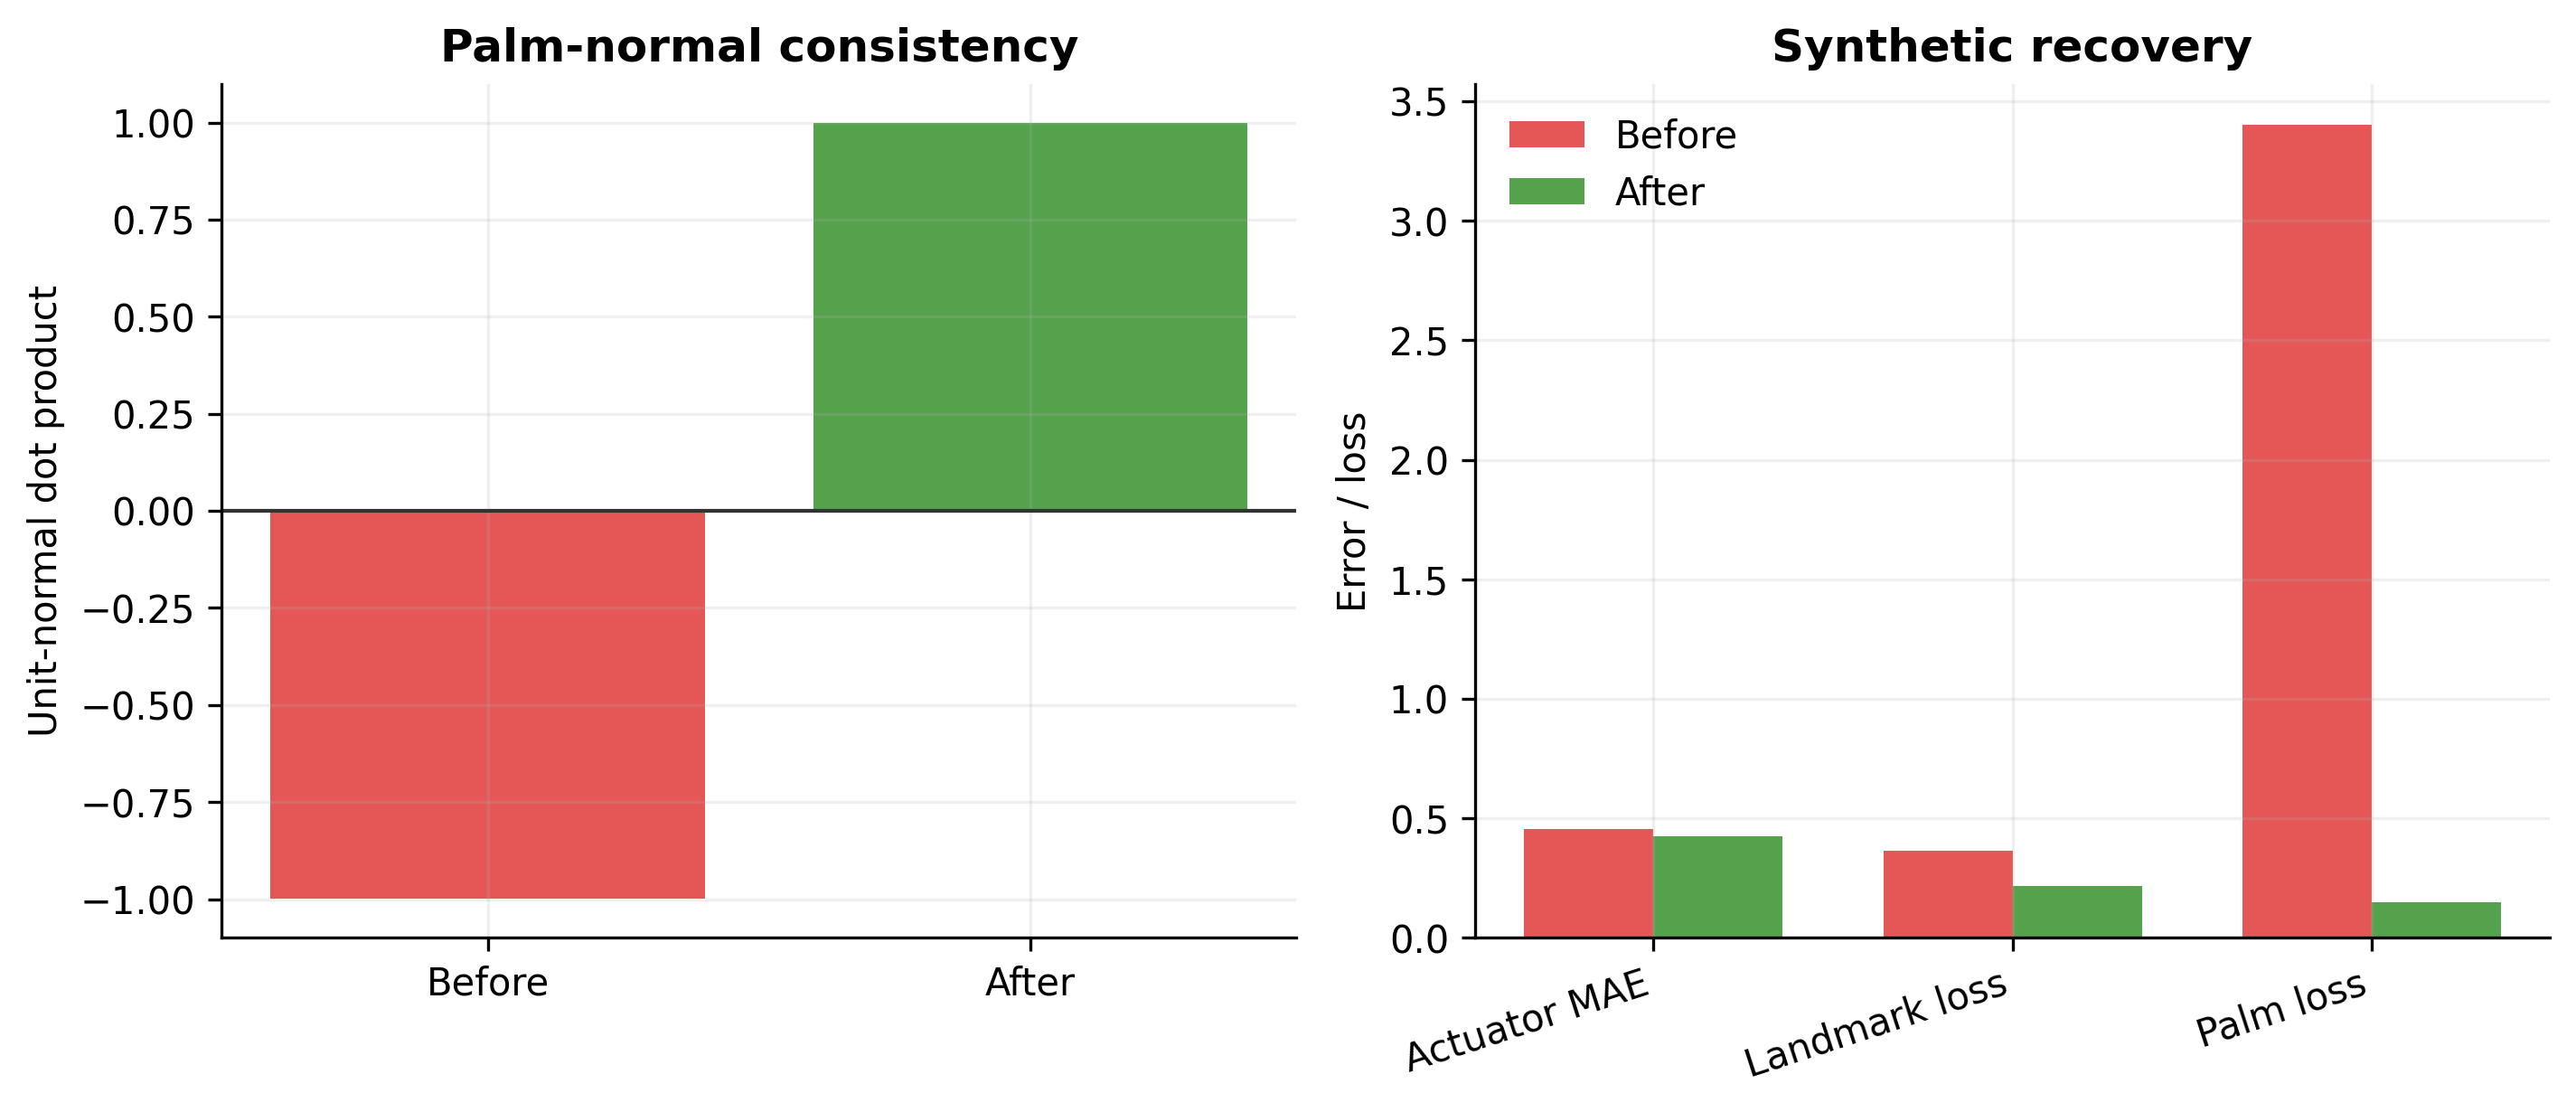
\includegraphics[width=0.82\linewidth]{paper_updated_6class_20260820/implementation_validation_before_after.png}
\caption{Implementation validation of the consistent palm-normal convention. The MuJoCo-generated target and predicted normals align after the correction, while synthetic actuator and landmark recovery errors decrease. This diagnostic validates the objective implementation rather than constituting a separate recognition baseline.}
\label{fig:implementation_validation_appendix}
\end{figure}

\bibliographystyle{ieeetr}
\bibliography{references}

\end{document}
